\chapter{Compiling the model and running a test case}\label{compile}

\vk
This chapter is meant for first time users of the LMD Martian Mesoscale Model. We describe how to compile the program and run a test case. We start with important basics about how the model works and how it is organized.

\mk
\section{Basics}

\sk
\subsection{Necessary steps to run a simulation}\label{steps}

\sk
Any simulation that will be carried out with the LMD Martian Mesoscale Model comprises the five following steps. More details are given on these steps in the following chapters, but it is important at this stage to have this structure in mind. 

\sk 
\begin{itemize}
\item \textbf{Step 0} Compiling the model.
\item \textbf{Step 1} Running the LMD Global Circulation Model (GCM) to provide initial and boundary conditions for the mesoscale model.
\item \textbf{Step 2} Choosing the mesoscale limited-area domain of simulation. Running preprocessing programs to horizontally interpolate GCM meteorological fields and static data (topography, soil properties) to the chosen simulation domain.
\item \textbf{Step 3} Running preprocessing programs to vertically interpolate GCM meteorological fields and generate the initial and boundary conditions directly used by the mesoscale model.
\item \textbf{Step 4} Running the LMD Martian Mesoscale Model.
\end{itemize}

\sk
In this chapter, the general method to perform steps 0 and 4 is reviewed. Other steps are reviewed in chapter~\ref{zepreproc}; here the model is compiled and run for a test case with precomputed sample files for preprocessing steps 1, 2, 3. 

\sk
\subsection{Structure of the \ttt{LMD\_MM\_MARS} directory}

\sk
Please take the time to check the contents of the \ttt{LMD\_MM\_MARS} directories\footnote{If you used method~$2$, you will probably notice that other directories than~\ttt{LMD\_MM\_MARS} are present in \ttt{\$MESO}, but those are not important at this stage.} and sub-directories through the following command lines:
\begin{verbatim}
ls $MMM ; ls $MMM/*
\end{verbatim}

\sk
Contents of~\ttt{LMD\_MM\_MARS} directory:
\begin{citemize}
\item \ttt{makemeso}: this is the \ttt{bash} script to compile the model.
\item \ttt{SRC}: this is a directory containing the model sources.
\item \ttt{SIMU}: this is a directory containing scripts and files for an advanced use.
\item \ttt{WPS\_GEOG}: this is a directory containing static data used in step~2.
\end{citemize}

\sk
Contents of~\ttt{LMD\_MM\_MARS/SRC} subdirectory:
\begin{citemize}
\item \ttt{SCRIPTS}: this is a directory containing useful \ttt{bash} scripts for installation.
\item \ttt{WRFV2}: this is a directory containing main model sources (modified WRF dynamics + LMD physics in \ttt{mars\_lmd*}).
\item \ttt{PREP\_MARS}: this is a directory containing sources for the last part of step~1.
\item \ttt{WPS}: this is a directory containing sources for step~2.
\item \ttt{POSTPROC}: this is a directory containing postprocessing sources.
%\item \ttt{PYTHON}: this is a directory containing \ttt{python}-based graphical scripts.
\item \ttt{LES} and \ttt{LESnophys\_}: these are directories containing sources for Large-Eddy Simulations.
\end{citemize}

\sk
Contents of~\ttt{LMD\_MM\_MARS/SIMU} subdirectory:
\begin{citemize}
\item \ttt{callphys.def},\ttt{dustopacity.def}, \ttt{run.def}, \ttt{namelist.input\_full}, \ttt{namelist.input\_minim}, \ttt{namelist.input\_nests}, \ttt{namelist.input\_les}, \ttt{namelist.wps\_example}, \ttt{namelist.wps\_nests}, \ttt{namelist.wps.template}~: these are useful example and template files to guide you through setting up your own parameters for the LMD Martian Mesoscale Model simulations. 
\item \ttt{calendar}: this is a text file containing time management information in the model.
\item \ttt{runmeso}: this is a \ttt{bash} script that can be used once the model and preprocessing systems are installed; it prepares and runs a mesoscale simulation by going from step~1 to~4. 
\item \ttt{RUN}: this is a directory containing various files and scripts useful for advanced simulations.
\item \ttt{DEF}: this is a directory containing many examples of parameter files for simulations.
\end{citemize}

\sk
\begin{finger}
\item In pre-2011 versions of the model, the contents of the various directories listed here might differ. This has probably no impact on your use of the model if you ensure the following files and directories are present in \ttt{LMD\_MM\_MARS}:
\begin{citemize}
\item \ttt{makemeso}, \ttt{prepare}, \ttt{prepare\_ini}, \ttt{copy\_model}
\item \ttt{SRC/WRFV2}, \ttt{SRC/PREP\_MARS}, \ttt{SRC/WPS}
\item \ttt{SIMU/runmeso}, \ttt{SIMU/calendar}
\item \ttt{WPS\_GEOG}
\end{citemize}
\end{finger}

\mk
\section{Main compilation step}
\label{sc:makemeso}

\sk
\subsection{Description of the \ttt{makemeso} script}

\sk
The \ttt{bash} script which allows you to compile the LMD Martian Mesoscale Model is \ttt{makemeso}. It is an automated script which performs the following serie of tasks:
\begin{citemize}
\item ask the user about compilation settings;
\item retrieve some additional information about the system;
\item create a directory \ttt{\$MESO/LMD\_MM\_MARS/your\_compdir} which name depends\footnote{For example, a \ttt{your\_compdir} directory named \ttt{g95\_32\_single} is created if the user requested a \ttt{g95} compilation of the code for single-domain simulations on a 32 bits machine.} on the kind of compiler you are using, on whether your system is 32 or 64 bits, on whether sequential or parallel computations are planned and on the kind of simulations (idealized or real-case); 
\item generate with \ttt{copy\_model} a directory \ttt{your\_compdir/WRFV2} with links to \ttt{SRC/WRFV2} sources\footnote{A note to developers: this method ensures that any change to the model sources would be propagated to all the different \ttt{your\_compdir} installation folders.};
\item execute the WRF \ttt{configure} script with the correct options;
\item tweak the resulting \ttt{configure.wrf} file to include a link towards the Martian physics and various patches and specific compilation options;
\item calculate the total number of horizontal grid points handled by the LMD physics;
\item duplicate LMD physical sources if nesting is activated;
\pagebreak
\item compile the LMD physical packages with the appropriate \ttt{makegcm} command
and collect the compiled objects in the library \ttt{liblmd.a};
\begin{finger}
\item This step could be a bit long, especially if you are defining more than one domain. The \ttt{makemeso} script provides you with the full path towards the text file \ttt{log\_compile\_phys} in which you can check for compilation progress and possible errors. In the end of the process, you might find at the end of~\ttt{log\_compile\_phys} an error message associated to the generation of the final executable. Please do not pay attention to this, as the compilation of the LMD sources is meant to generate a library of compiled objects called \ttt{liblmd.a} instead of an executable.
\end{finger}
\item compile the modified Martian ARW-WRF solver and include the \ttt{liblmd.a} library; 
\begin{finger}
\item When it is the first time the model is compiled, this step could be quite long. The \ttt{makemeso} script provides you with a \ttt{log\_compile} text file where the progress of the compilation can be checked and a \ttt{log\_error} text file listing errors and warnings during compilation. A list of warnings related to \ttt{grib} utilities (not used in the Martian model) may appear and have no impact on the final executables.
\end{finger}
\item change the name of the executables in agreement with the
settings provided by the user.
\end{citemize}

\sk
\subsection{Use of the \ttt{makemeso} script}

\sk
To compile the model, change directory to \ttt{\$MMM} and execute the \ttt{makemeso} command:

\begin{verbatim}
cd $MMM
./makemeso
\end{verbatim}

\sk
You are asked a few questions by the \ttt{makemeso} script (see the list below) then it compiles the model for you. The script outputs a text file named \ttt{last} in which your answers to the questions are stored, which allows you to re-run the script without the ``questions to the user" step through the \ttt{makemeso < last} command line. 

\mk
\begin{asparaenum}[1.]%[\itshape Q1\upshape)]
\item \textbf{choice of compiler}\footnote{We advise you to compile the model on the same kind of system (computer + operating system + librairies) as the one you plan to use to run the model.} 
\item[1.bis] (mpi-based compilation) number of processors to be used
\item \textbf{number of grid points in longitude}\footnote{When you use parallel computations, please bear in mind that with $2$ (respectively $4$, $6$, $8$, $12$, $16$, $20$, $24$, $32$, $64$, $128$) processors the whole domain would be separated into $1$ (resp. $2$, $2$, $2$,  $3$,  $4$,  $4$,  $4$,  $4$,  $8$,   $8$) tiles over the longitude direction and $2$ (resp. $2$, $3$, $4$,  $4$,  $4$,  $5$,  $6$,  $8$,  $8$,  $16$) tiles over the latitude direction. Thus make sure that the number of grid points minus $1$ in each direction could be divided by the aforementioned number of tiles over the considered direction. For instance a~$82 \times 109$ horizontal grid is compliant with the use of~$12$ processors.} [61]
\item \textbf{number of grid points in latitude} [61]
\item \textbf{number of vertical levels} [61] 
\item \textbf{number of tracers}\footnote{The minimum number of tracers is 1 and not 0. Setting to 0 will actually make the script to set tracer number to 1.} [1]
\item \textbf{number of domains} [1]
%\item[6.bis] (not the first time you use \ttt{makemeso}) a question for advanced users [press any key]
%\item[6.ter] (new LMD physics) number of different scatterers to be used
\end{asparaenum}

\sk
The answers given in brackets above are the ones you want to use so that you will be able to run the test case proposed in the next section. Otherwise, before proceeding with \ttt{makemeso}, it is good to get used to gather the following information
\begin{itemize}
\item On which machine do you want to run the model? (a good practice is to compile on the same machine as the one used to run the model).
\item What is the horizontal resolution you want for your simulation? How many domains? How many tracers?
\item If parallel computations are employed: Do you have parallel librairies installed on the machine you chose? How much processors you want to use? 
\end{itemize}

\mk
A key question that often arises when using the LMD Martian Mesoscale Model is: when does the model has to be recompiled? The set of questions asked by~\ttt{makemeso} give some hints about this. Suppose you compiled a version of the model for a given set of parameters $1$ to $6$ to run a specific compilation. If you would like to run another simulation with at least one of parameters $1$ to $6$ subject to change, the model needs to be recompiled\footnote{This necessary recompilation each time the number of grid points, tracers and domains is modified is imposed by the LMD physics code. The WRF dynamical core alone is more flexible.} with \ttt{makemeso} (cf. also chapter~\ref{zeparam}).

\mk
Note that the \ttt{makemeso -h} command lists the various options that can be used in the \ttt{makemeso} script. Most options should be used only by advanced users and some of them will be described in the following chapters. At this stage, the only option of \ttt{makemeso} which can be useful to you is \ttt{-f} which forces the model to be recompiled from scratch (this is for instance very useful if a previous compilation ran into problems, or was interrupted by the user). If you already compiled the model succesfully, but the model fails to compile a few days later for reasons unrelated to your operations on your system or on the model file, we recommend you to use the \ttt{-f} option in \ttt{makemeso} to try to recompile the model\footnote{A more extreme solution if \ttt{makemeso -f} does not solve your problem is to remove the corresponding \ttt{your\_compdir} directory. See chapter~\ref{faq}}.

\scriptsize
\codesource{makemesohelp}
\normalsize

\mk
\section{Running a simple test case}
\label{sc:arsia}

\sk
We assume here that you had successfully compiled the model with \ttt{makemeso} at the end of the previous section and you had based your answers to the \ttt{makemeso} script on the indications in brackets. You should then find in the \ttt{your\_compdir} directory the \ttt{real\_x61\_y61\_z61\_d1\_t1\_p1.exe} and~\ttt{wrf\_x61\_y61\_z61\_d1\_t1\_p1.exe} executables.

\sk
In order to test the compiled executables, a ready-to-use test case (with pre-generated initial and boundary conditions) is proposed in the \ttt{LMD\_MM\_MARS/SIMU/DEF/TESTCASE} folder (use the \ttt{EXEC\_TO\_GET\_data.sh} command to get the initial and boundary condition files). This test case simulates the hydrostatic atmospheric flow around Arsia Mons (Figure~\ref{arsia}) during half a sol in springtime with constant thermal inertia, albedo and dust opacity\footnote{Though the simulation reproduces some reasonable features of the mesoscale circulation around Arsia Mons (e.g. slope winds), it should not be used for scientific purpose, for the number of grid points is unsufficient for single-domain simulation and the integration time is below the necessary spin-up time.}.

\sk
To launch the test simulation, please type the following commands, replacing if needed the \ttt{LATEST} directory with its corresponding value on your system. In the end, the model should run and output the computed meteorological fields in netCDF files named \ttt{wrfout*}. Feel free to browse those files with \ttt{ncview} or your favorite graphical tool to check if the simulated fields look reasonable. 
%
\begin{verbatim}
cd $MMM/SIMU/DEF/TESTCASE
./EXEC_TO_GET_data.sh (only once)
ln -sf ../../../LATEST/wrf_x61_y61_z61_d1_t1_p1.exe wrf.exe  
nohup wrf.exe > log_wrf &
\end{verbatim}

\sk
The files contained in \ttt{TESTCASE} prior to launching the simulations with the \ttt{wrf.exe} command illustrate which files are needed to perform step 4, i.e. running a LMD Martian Mesoscale Model simulation\footnote{For the test case presented here, a file named \ttt{dustopacity.def} is needed because for the sake of simplicity of this test case, we set idealized uniform dust opacity. The file \ttt{namelist.wps} is included in the \ttt{TESTCASE} folder for further reference but not needed at this stage.}. 
\begin{itemize}
\item \ttt{namelist.input}: text file containing parameters for the dynamical core
\item \ttt{callphys.def}: text file containing parameters for the physics parameterizations
\item \ttt{wrf.exe}: the model executable (or a link to it) as compiled by \ttt{makemeso}
\item \ttt{wrfinput\_d01} and \ttt{wrfbdy\_d01}: data files containing initial and boundary conditions
\end{itemize}

\begin{center} 
\begin{figure}[h!]
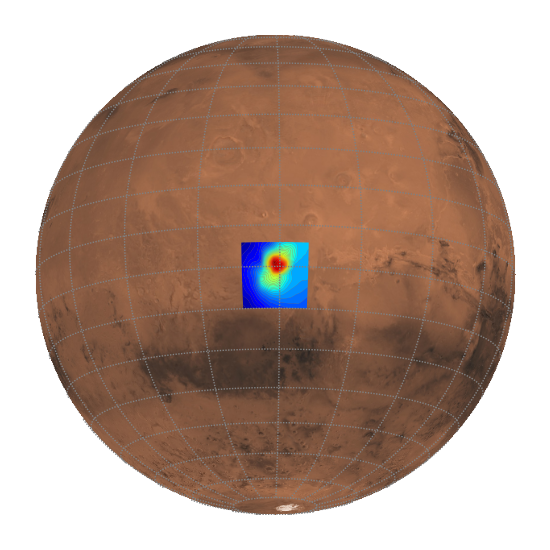
\includegraphics[width=0.5\textwidth]{arsiadomain.png} 
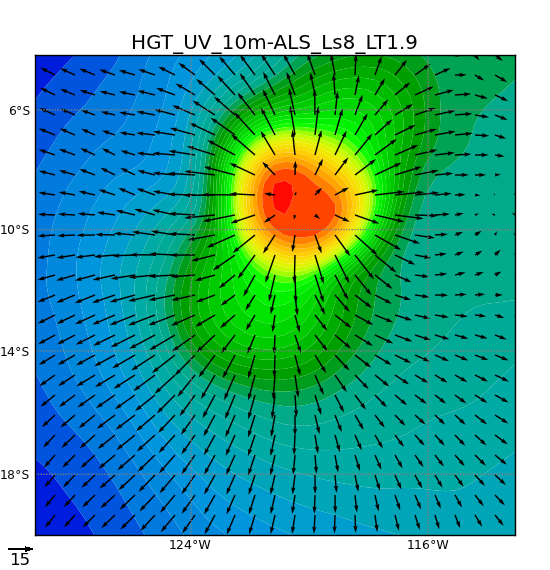
\includegraphics[width=0.5\textwidth]{LMD_MMM_d1_20km_HGT_UV_10m-ALS_Ls8_LT1_100.png}
\caption{\label{arsia} [Left plot] Simulation domain defined in the test case proposed as a demonstrator for running the LMD Martian Mesoscale Model. [Right plot] Nighttime winds predicted by the model~$10$~m above the surface. Both plots have been generated by command-line scripts written in~\ttt{python + numpy + matplotlib} (see chapter~\ref{postproc}).}
\end{figure}
\end{center}

\bk
%\scriptsize
\begin{finger}
\item If you compiled the model using MPI, the command to launch a simulation is slightly different:
%
\begin{verbatim}
[if several connected machines, create a file mpd.hosts with machine names...]
[... and make sure that ssh between machines does not need authentification]
mpirun [-f mpd.hosts] -np number_of_processors wrf.exe < /dev/null &      
tail -20 rsl.out.000? # to check the outputs
\end{verbatim}
%%echo barry.lmd.jussieu.fr > ~/mpd.hosts
%%echo white.lmd.jussieu.fr >> ~/mpd.hosts
%%echo loves.lmd.jussieu.fr >> ~/mpd.hosts
%%echo tapas.lmd.jussieu.fr >> ~/mpd.hosts	
%%mpdboot  -n 4
%%mpdtrace
%%mpirun -l -np 16 wrf.exe < /dev/null &   # NB: mpirun is only a link to mpiexec
\end{finger}
%\normalsize

\clearemptydoublepage
